\begin{figure}[t]
\uwsinglespace
\begin{center}
\begin{minipage}{0.45\textwidth}
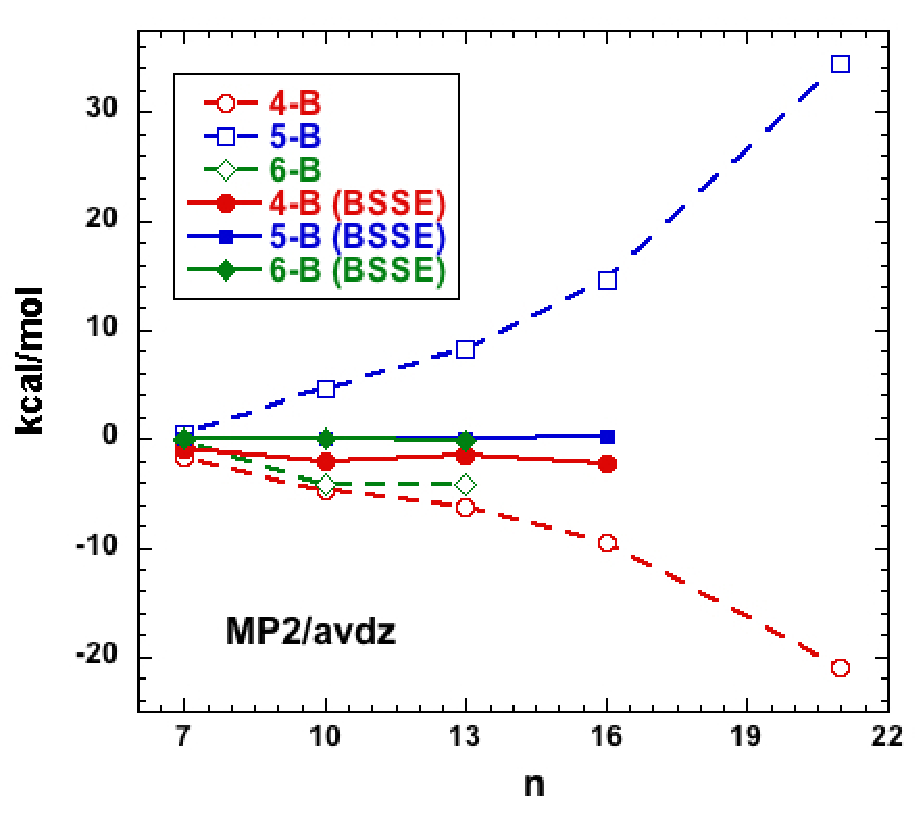
\includegraphics[width=\textwidth]{Figures/Chapter_2/4_B_6_B_vs_n.pdf}
\end{minipage}
\begin{minipage}{0.45\textwidth}
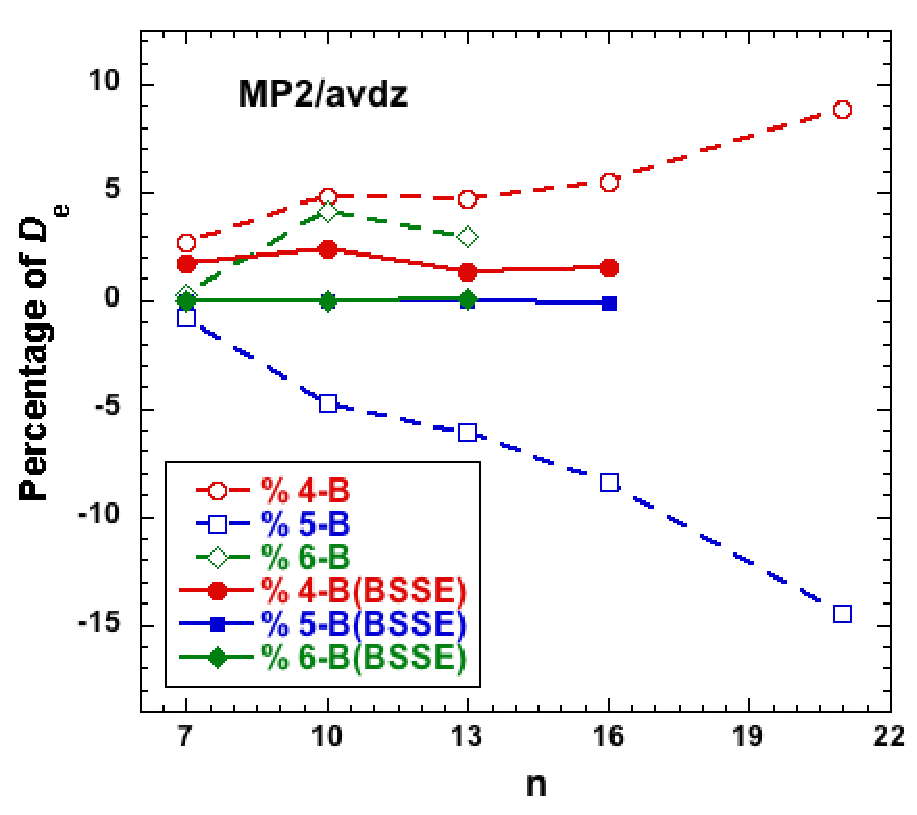
\includegraphics[width=\textwidth]{Figures/Chapter_2/4_B_6_B_perc_vs_n.pdf}
\end{minipage}
\end{center}
\begin{spacing}{1.0}
\caption[The absolute magnitudes (left) and percentage contributions (right) of the 4- to 6-body terms to the MP2/AVDZ binding energy for (H2O)n, n = 7, 10, 13, 16 and 21. The uncorrected (dashed lines) and BSSE-corrected results (solid lines) are shown.]{The absolute magnitudes (left) and percentage contributions (right) of the 4- to 6-body terms to the MP2/AVDZ binding energy for (H2O)n, n = 7, 10, 13, 16 and 21. The uncorrected (dashed lines) and BSSE-corrected results (solid lines) are shown.}\label{fig:MBE_I_F5}
\end{spacing}
\end{figure}